\documentclass{article} % For LaTeX2e
\usepackage{iclr2023_conference, times}

\usepackage[utf8]{inputenc} % allow utf-8 input
\usepackage[T1]{fontenc}    % use 8-bit T1 fonts
\usepackage{hyperref}       % hyperlinks
\usepackage{url}            % simple URL typesetting
\usepackage{booktabs}       % professional-quality tables
\usepackage{amsfonts}       % blackboard math symbols
\usepackage{nicefrac}       % compact symbols for 1/2, etc.
\usepackage{microtype}      % microtypography
\usepackage{xcolor}         % colors

% --- Custom formatting --- 
% images
\setcounter{topnumber}{2}
\setcounter{bottomnumber}{2}
\setcounter{totalnumber}{4}
\renewcommand{\topfraction}{0.85}
\renewcommand{\bottomfraction}{0.85}
\renewcommand{\textfraction}{0.15}
\renewcommand{\floatpagefraction}{0.8}
\renewcommand{\textfraction}{0.1}
\setlength{\floatsep}{5pt plus 2pt minus 2pt}
\setlength{\textfloatsep}{5pt plus 2pt minus 2pt}
\setlength{\intextsep}{5pt plus 2pt minus 2pt}
\setlength{\abovedisplayskip}{0pt}
\setlength{\belowdisplayskip}{0pt}
\setlength{\abovedisplayshortskip}{0pt}
\setlength{\belowdisplayshortskip}{0pt}

% text
\usepackage{titlesec}

\titlespacing*{\section}
{0pt}{.2cm}{.1cm}
\titlespacing*{\subsection}
{0pt}{.1cm}{.1cm}

% --- Default packages --- 
% Optional math commands from https://github.com/goodfeli/dlbook_notation.
%%%%% NEW MATH DEFINITIONS %%%%%

\usepackage{amsmath,amsfonts,bm}

% Mark sections of captions for referring to divisions of figures
\newcommand{\figleft}{{\em (Left)}}
\newcommand{\figcenter}{{\em (Center)}}
\newcommand{\figright}{{\em (Right)}}
\newcommand{\figtop}{{\em (Top)}}
\newcommand{\figbottom}{{\em (Bottom)}}
\newcommand{\captiona}{{\em (a)}}
\newcommand{\captionb}{{\em (b)}}
\newcommand{\captionc}{{\em (c)}}
\newcommand{\captiond}{{\em (d)}}

% Highlight a newly defined term
\newcommand{\newterm}[1]{{\bf #1}}


% Figure reference, lower-case.
\def\figref#1{figure~\ref{#1}}
% Figure reference, capital. For start of sentence
\def\Figref#1{Figure~\ref{#1}}
\def\twofigref#1#2{figures \ref{#1} and \ref{#2}}
\def\quadfigref#1#2#3#4{figures \ref{#1}, \ref{#2}, \ref{#3} and \ref{#4}}
% Section reference, lower-case.
\def\secref#1{section~\ref{#1}}
% Section reference, capital.
\def\Secref#1{Section~\ref{#1}}
% Reference to two sections.
\def\twosecrefs#1#2{sections \ref{#1} and \ref{#2}}
% Reference to three sections.
\def\secrefs#1#2#3{sections \ref{#1}, \ref{#2} and \ref{#3}}
% Reference to an equation, lower-case.
\def\eqref#1{equation~\ref{#1}}
% Reference to an equation, upper case
\def\Eqref#1{Equation~\ref{#1}}
% A raw reference to an equation---avoid using if possible
\def\plaineqref#1{\ref{#1}}
% Reference to a chapter, lower-case.
\def\chapref#1{chapter~\ref{#1}}
% Reference to an equation, upper case.
\def\Chapref#1{Chapter~\ref{#1}}
% Reference to a range of chapters
\def\rangechapref#1#2{chapters\ref{#1}--\ref{#2}}
% Reference to an algorithm, lower-case.
\def\algref#1{algorithm~\ref{#1}}
% Reference to an algorithm, upper case.
\def\Algref#1{Algorithm~\ref{#1}}
\def\twoalgref#1#2{algorithms \ref{#1} and \ref{#2}}
\def\Twoalgref#1#2{Algorithms \ref{#1} and \ref{#2}}
% Reference to a part, lower case
\def\partref#1{part~\ref{#1}}
% Reference to a part, upper case
\def\Partref#1{Part~\ref{#1}}
\def\twopartref#1#2{parts \ref{#1} and \ref{#2}}

\def\ceil#1{\lceil #1 \rceil}
\def\floor#1{\lfloor #1 \rfloor}
\def\1{\bm{1}}
\newcommand{\train}{\mathcal{D}}
\newcommand{\valid}{\mathcal{D_{\mathrm{valid}}}}
\newcommand{\test}{\mathcal{D_{\mathrm{test}}}}

\def\eps{{\epsilon}}


% Random variables
\def\reta{{\textnormal{$\eta$}}}
\def\ra{{\textnormal{a}}}
\def\rb{{\textnormal{b}}}
\def\rc{{\textnormal{c}}}
\def\rd{{\textnormal{d}}}
\def\re{{\textnormal{e}}}
\def\rf{{\textnormal{f}}}
\def\rg{{\textnormal{g}}}
\def\rh{{\textnormal{h}}}
\def\ri{{\textnormal{i}}}
\def\rj{{\textnormal{j}}}
\def\rk{{\textnormal{k}}}
\def\rl{{\textnormal{l}}}
% rm is already a command, just don't name any random variables m
\def\rn{{\textnormal{n}}}
\def\ro{{\textnormal{o}}}
\def\rp{{\textnormal{p}}}
\def\rq{{\textnormal{q}}}
\def\rr{{\textnormal{r}}}
\def\rs{{\textnormal{s}}}
\def\rt{{\textnormal{t}}}
\def\ru{{\textnormal{u}}}
\def\rv{{\textnormal{v}}}
\def\rw{{\textnormal{w}}}
\def\rx{{\textnormal{x}}}
\def\ry{{\textnormal{y}}}
\def\rz{{\textnormal{z}}}

% Random vectors
\def\rvepsilon{{\mathbf{\epsilon}}}
\def\rvtheta{{\mathbf{\theta}}}
\def\rva{{\mathbf{a}}}
\def\rvb{{\mathbf{b}}}
\def\rvc{{\mathbf{c}}}
\def\rvd{{\mathbf{d}}}
\def\rve{{\mathbf{e}}}
\def\rvf{{\mathbf{f}}}
\def\rvg{{\mathbf{g}}}
\def\rvh{{\mathbf{h}}}
\def\rvu{{\mathbf{i}}}
\def\rvj{{\mathbf{j}}}
\def\rvk{{\mathbf{k}}}
\def\rvl{{\mathbf{l}}}
\def\rvm{{\mathbf{m}}}
\def\rvn{{\mathbf{n}}}
\def\rvo{{\mathbf{o}}}
\def\rvp{{\mathbf{p}}}
\def\rvq{{\mathbf{q}}}
\def\rvr{{\mathbf{r}}}
\def\rvs{{\mathbf{s}}}
\def\rvt{{\mathbf{t}}}
\def\rvu{{\mathbf{u}}}
\def\rvv{{\mathbf{v}}}
\def\rvw{{\mathbf{w}}}
\def\rvx{{\mathbf{x}}}
\def\rvy{{\mathbf{y}}}
\def\rvz{{\mathbf{z}}}

% Elements of random vectors
\def\erva{{\textnormal{a}}}
\def\ervb{{\textnormal{b}}}
\def\ervc{{\textnormal{c}}}
\def\ervd{{\textnormal{d}}}
\def\erve{{\textnormal{e}}}
\def\ervf{{\textnormal{f}}}
\def\ervg{{\textnormal{g}}}
\def\ervh{{\textnormal{h}}}
\def\ervi{{\textnormal{i}}}
\def\ervj{{\textnormal{j}}}
\def\ervk{{\textnormal{k}}}
\def\ervl{{\textnormal{l}}}
\def\ervm{{\textnormal{m}}}
\def\ervn{{\textnormal{n}}}
\def\ervo{{\textnormal{o}}}
\def\ervp{{\textnormal{p}}}
\def\ervq{{\textnormal{q}}}
\def\ervr{{\textnormal{r}}}
\def\ervs{{\textnormal{s}}}
\def\ervt{{\textnormal{t}}}
\def\ervu{{\textnormal{u}}}
\def\ervv{{\textnormal{v}}}
\def\ervw{{\textnormal{w}}}
\def\ervx{{\textnormal{x}}}
\def\ervy{{\textnormal{y}}}
\def\ervz{{\textnormal{z}}}

% Random matrices
\def\rmA{{\mathbf{A}}}
\def\rmB{{\mathbf{B}}}
\def\rmC{{\mathbf{C}}}
\def\rmD{{\mathbf{D}}}
\def\rmE{{\mathbf{E}}}
\def\rmF{{\mathbf{F}}}
\def\rmG{{\mathbf{G}}}
\def\rmH{{\mathbf{H}}}
\def\rmI{{\mathbf{I}}}
\def\rmJ{{\mathbf{J}}}
\def\rmK{{\mathbf{K}}}
\def\rmL{{\mathbf{L}}}
\def\rmM{{\mathbf{M}}}
\def\rmN{{\mathbf{N}}}
\def\rmO{{\mathbf{O}}}
\def\rmP{{\mathbf{P}}}
\def\rmQ{{\mathbf{Q}}}
\def\rmR{{\mathbf{R}}}
\def\rmS{{\mathbf{S}}}
\def\rmT{{\mathbf{T}}}
\def\rmU{{\mathbf{U}}}
\def\rmV{{\mathbf{V}}}
\def\rmW{{\mathbf{W}}}
\def\rmX{{\mathbf{X}}}
\def\rmY{{\mathbf{Y}}}
\def\rmZ{{\mathbf{Z}}}

% Elements of random matrices
\def\ermA{{\textnormal{A}}}
\def\ermB{{\textnormal{B}}}
\def\ermC{{\textnormal{C}}}
\def\ermD{{\textnormal{D}}}
\def\ermE{{\textnormal{E}}}
\def\ermF{{\textnormal{F}}}
\def\ermG{{\textnormal{G}}}
\def\ermH{{\textnormal{H}}}
\def\ermI{{\textnormal{I}}}
\def\ermJ{{\textnormal{J}}}
\def\ermK{{\textnormal{K}}}
\def\ermL{{\textnormal{L}}}
\def\ermM{{\textnormal{M}}}
\def\ermN{{\textnormal{N}}}
\def\ermO{{\textnormal{O}}}
\def\ermP{{\textnormal{P}}}
\def\ermQ{{\textnormal{Q}}}
\def\ermR{{\textnormal{R}}}
\def\ermS{{\textnormal{S}}}
\def\ermT{{\textnormal{T}}}
\def\ermU{{\textnormal{U}}}
\def\ermV{{\textnormal{V}}}
\def\ermW{{\textnormal{W}}}
\def\ermX{{\textnormal{X}}}
\def\ermY{{\textnormal{Y}}}
\def\ermZ{{\textnormal{Z}}}

% Vectors
\def\vzero{{\bm{0}}}
\def\vone{{\bm{1}}}
\def\vmu{{\bm{\mu}}}
\def\vtheta{{\bm{\theta}}}
\def\va{{\bm{a}}}
\def\vb{{\bm{b}}}
\def\vc{{\bm{c}}}
\def\vd{{\bm{d}}}
\def\ve{{\bm{e}}}
\def\vf{{\bm{f}}}
\def\vg{{\bm{g}}}
\def\vh{{\bm{h}}}
\def\vi{{\bm{i}}}
\def\vj{{\bm{j}}}
\def\vk{{\bm{k}}}
\def\vl{{\bm{l}}}
\def\vm{{\bm{m}}}
\def\vn{{\bm{n}}}
\def\vo{{\bm{o}}}
\def\vp{{\bm{p}}}
\def\vq{{\bm{q}}}
\def\vr{{\bm{r}}}
\def\vs{{\bm{s}}}
\def\vt{{\bm{t}}}
\def\vu{{\bm{u}}}
\def\vv{{\bm{v}}}
\def\vw{{\bm{w}}}
\def\vx{{\bm{x}}}
\def\vy{{\bm{y}}}
\def\vz{{\bm{z}}}

% Elements of vectors
\def\evalpha{{\alpha}}
\def\evbeta{{\beta}}
\def\evepsilon{{\epsilon}}
\def\evlambda{{\lambda}}
\def\evomega{{\omega}}
\def\evmu{{\mu}}
\def\evpsi{{\psi}}
\def\evsigma{{\sigma}}
\def\evtheta{{\theta}}
\def\eva{{a}}
\def\evb{{b}}
\def\evc{{c}}
\def\evd{{d}}
\def\eve{{e}}
\def\evf{{f}}
\def\evg{{g}}
\def\evh{{h}}
\def\evi{{i}}
\def\evj{{j}}
\def\evk{{k}}
\def\evl{{l}}
\def\evm{{m}}
\def\evn{{n}}
\def\evo{{o}}
\def\evp{{p}}
\def\evq{{q}}
\def\evr{{r}}
\def\evs{{s}}
\def\evt{{t}}
\def\evu{{u}}
\def\evv{{v}}
\def\evw{{w}}
\def\evx{{x}}
\def\evy{{y}}
\def\evz{{z}}

% Matrix
\def\mA{{\bm{A}}}
\def\mB{{\bm{B}}}
\def\mC{{\bm{C}}}
\def\mD{{\bm{D}}}
\def\mE{{\bm{E}}}
\def\mF{{\bm{F}}}
\def\mG{{\bm{G}}}
\def\mH{{\bm{H}}}
\def\mI{{\bm{I}}}
\def\mJ{{\bm{J}}}
\def\mK{{\bm{K}}}
\def\mL{{\bm{L}}}
\def\mM{{\bm{M}}}
\def\mN{{\bm{N}}}
\def\mO{{\bm{O}}}
\def\mP{{\bm{P}}}
\def\mQ{{\bm{Q}}}
\def\mR{{\bm{R}}}
\def\mS{{\bm{S}}}
\def\mT{{\bm{T}}}
\def\mU{{\bm{U}}}
\def\mV{{\bm{V}}}
\def\mW{{\bm{W}}}
\def\mX{{\bm{X}}}
\def\mY{{\bm{Y}}}
\def\mZ{{\bm{Z}}}
\def\mBeta{{\bm{\beta}}}
\def\mPhi{{\bm{\Phi}}}
\def\mLambda{{\bm{\Lambda}}}
\def\mSigma{{\bm{\Sigma}}}

% Tensor
\DeclareMathAlphabet{\mathsfit}{\encodingdefault}{\sfdefault}{m}{sl}
\SetMathAlphabet{\mathsfit}{bold}{\encodingdefault}{\sfdefault}{bx}{n}
\newcommand{\tens}[1]{\bm{\mathsfit{#1}}}
\def\tA{{\tens{A}}}
\def\tB{{\tens{B}}}
\def\tC{{\tens{C}}}
\def\tD{{\tens{D}}}
\def\tE{{\tens{E}}}
\def\tF{{\tens{F}}}
\def\tG{{\tens{G}}}
\def\tH{{\tens{H}}}
\def\tI{{\tens{I}}}
\def\tJ{{\tens{J}}}
\def\tK{{\tens{K}}}
\def\tL{{\tens{L}}}
\def\tM{{\tens{M}}}
\def\tN{{\tens{N}}}
\def\tO{{\tens{O}}}
\def\tP{{\tens{P}}}
\def\tQ{{\tens{Q}}}
\def\tR{{\tens{R}}}
\def\tS{{\tens{S}}}
\def\tT{{\tens{T}}}
\def\tU{{\tens{U}}}
\def\tV{{\tens{V}}}
\def\tW{{\tens{W}}}
\def\tX{{\tens{X}}}
\def\tY{{\tens{Y}}}
\def\tZ{{\tens{Z}}}


% Graph
\def\gA{{\mathcal{A}}}
\def\gB{{\mathcal{B}}}
\def\gC{{\mathcal{C}}}
\def\gD{{\mathcal{D}}}
\def\gE{{\mathcal{E}}}
\def\gF{{\mathcal{F}}}
\def\gG{{\mathcal{G}}}
\def\gH{{\mathcal{H}}}
\def\gI{{\mathcal{I}}}
\def\gJ{{\mathcal{J}}}
\def\gK{{\mathcal{K}}}
\def\gL{{\mathcal{L}}}
\def\gM{{\mathcal{M}}}
\def\gN{{\mathcal{N}}}
\def\gO{{\mathcal{O}}}
\def\gP{{\mathcal{P}}}
\def\gQ{{\mathcal{Q}}}
\def\gR{{\mathcal{R}}}
\def\gS{{\mathcal{S}}}
\def\gT{{\mathcal{T}}}
\def\gU{{\mathcal{U}}}
\def\gV{{\mathcal{V}}}
\def\gW{{\mathcal{W}}}
\def\gX{{\mathcal{X}}}
\def\gY{{\mathcal{Y}}}
\def\gZ{{\mathcal{Z}}}

% Sets
\def\sA{{\mathbb{A}}}
\def\sB{{\mathbb{B}}}
\def\sC{{\mathbb{C}}}
\def\sD{{\mathbb{D}}}
% Don't use a set called E, because this would be the same as our symbol
% for expectation.
\def\sF{{\mathbb{F}}}
\def\sG{{\mathbb{G}}}
\def\sH{{\mathbb{H}}}
\def\sI{{\mathbb{I}}}
\def\sJ{{\mathbb{J}}}
\def\sK{{\mathbb{K}}}
\def\sL{{\mathbb{L}}}
\def\sM{{\mathbb{M}}}
\def\sN{{\mathbb{N}}}
\def\sO{{\mathbb{O}}}
\def\sP{{\mathbb{P}}}
\def\sQ{{\mathbb{Q}}}
\def\sR{{\mathbb{R}}}
\def\sS{{\mathbb{S}}}
\def\sT{{\mathbb{T}}}
\def\sU{{\mathbb{U}}}
\def\sV{{\mathbb{V}}}
\def\sW{{\mathbb{W}}}
\def\sX{{\mathbb{X}}}
\def\sY{{\mathbb{Y}}}
\def\sZ{{\mathbb{Z}}}

% Entries of a matrix
\def\emLambda{{\Lambda}}
\def\emA{{A}}
\def\emB{{B}}
\def\emC{{C}}
\def\emD{{D}}
\def\emE{{E}}
\def\emF{{F}}
\def\emG{{G}}
\def\emH{{H}}
\def\emI{{I}}
\def\emJ{{J}}
\def\emK{{K}}
\def\emL{{L}}
\def\emM{{M}}
\def\emN{{N}}
\def\emO{{O}}
\def\emP{{P}}
\def\emQ{{Q}}
\def\emR{{R}}
\def\emS{{S}}
\def\emT{{T}}
\def\emU{{U}}
\def\emV{{V}}
\def\emW{{W}}
\def\emX{{X}}
\def\emY{{Y}}
\def\emZ{{Z}}
\def\emSigma{{\Sigma}}

% entries of a tensor
% Same font as tensor, without \bm wrapper
\newcommand{\etens}[1]{\mathsfit{#1}}
\def\etLambda{{\etens{\Lambda}}}
\def\etA{{\etens{A}}}
\def\etB{{\etens{B}}}
\def\etC{{\etens{C}}}
\def\etD{{\etens{D}}}
\def\etE{{\etens{E}}}
\def\etF{{\etens{F}}}
\def\etG{{\etens{G}}}
\def\etH{{\etens{H}}}
\def\etI{{\etens{I}}}
\def\etJ{{\etens{J}}}
\def\etK{{\etens{K}}}
\def\etL{{\etens{L}}}
\def\etM{{\etens{M}}}
\def\etN{{\etens{N}}}
\def\etO{{\etens{O}}}
\def\etP{{\etens{P}}}
\def\etQ{{\etens{Q}}}
\def\etR{{\etens{R}}}
\def\etS{{\etens{S}}}
\def\etT{{\etens{T}}}
\def\etU{{\etens{U}}}
\def\etV{{\etens{V}}}
\def\etW{{\etens{W}}}
\def\etX{{\etens{X}}}
\def\etY{{\etens{Y}}}
\def\etZ{{\etens{Z}}}

% The true underlying data generating distribution
\newcommand{\pdata}{p_{\rm{data}}}
% The empirical distribution defined by the training set
\newcommand{\ptrain}{\hat{p}_{\rm{data}}}
\newcommand{\Ptrain}{\hat{P}_{\rm{data}}}
% The model distribution
\newcommand{\pmodel}{p_{\rm{model}}}
\newcommand{\Pmodel}{P_{\rm{model}}}
\newcommand{\ptildemodel}{\tilde{p}_{\rm{model}}}
% Stochastic autoencoder distributions
\newcommand{\pencode}{p_{\rm{encoder}}}
\newcommand{\pdecode}{p_{\rm{decoder}}}
\newcommand{\precons}{p_{\rm{reconstruct}}}

\newcommand{\laplace}{\mathrm{Laplace}} % Laplace distribution

\newcommand{\E}{\mathbb{E}}
\newcommand{\Ls}{\mathcal{L}}
\newcommand{\R}{\mathbb{R}}
\newcommand{\emp}{\tilde{p}}
\newcommand{\lr}{\alpha}
\newcommand{\reg}{\lambda}
\newcommand{\rect}{\mathrm{rectifier}}
\newcommand{\softmax}{\mathrm{softmax}}
\newcommand{\sigmoid}{\sigma}
\newcommand{\softplus}{\zeta}
\newcommand{\KL}{D_{\mathrm{KL}}}
\newcommand{\Var}{\mathrm{Var}}
\newcommand{\standarderror}{\mathrm{SE}}
\newcommand{\Cov}{\mathrm{Cov}}
% Wolfram Mathworld says $L^2$ is for function spaces and $\ell^2$ is for vectors
% But then they seem to use $L^2$ for vectors throughout the site, and so does
% wikipedia.
\newcommand{\normlzero}{L^0}
\newcommand{\normlone}{L^1}
\newcommand{\normltwo}{L^2}
\newcommand{\normlp}{L^p}
\newcommand{\normmax}{L^\infty}

\newcommand{\parents}{Pa} % See usage in notation.tex. Chosen to match Daphne's book.

\DeclareMathOperator*{\argmax}{arg\,max}
\DeclareMathOperator*{\argmin}{arg\,min}

\DeclareMathOperator{\sign}{sign}
\DeclareMathOperator{\Tr}{Tr}
\let\ab\allowbreak

\usepackage{hyperref}
\usepackage{url}

% --- Custom packages --- 
% images
\usepackage{graphicx}
\usepackage{float}
\usepackage{placeins}
\usepackage{wrapfig}
\usepackage{subcaption}
\usepackage[export]{adjustbox}

% psudeocode
\usepackage{algorithm}
\usepackage{algpseudocode}
\def\NoNumber#1{{\def\alglinenumber##1{}\State #1}\addtocounter{ALG@line}{-1}}

\newtheorem{theorem}{Theorem}
\newtheorem{definition}{Definition}
\newtheorem{lemma}{Lemma}
\newtheorem{prop}{Proposition}
\newcommand{\indep}{\perp \!\!\! \perp}

\newcommand{\yli}[1]{{\color{cyan}#1}}
\newcommand{\joe}[1]{\textcolor{blue}{#1}}
\newcommand{\cmh}[1]{\textcolor{orange}{\scriptsize Minhao: #1}}

\title{
    Trusted Aggregation (TAG): Model Filtering Backdoor Defense In Federated Learning
}

% Authors must not appear in the submitted version. They should be hidden
% as long as the \iclrfinalcopy macro remains commented out below.
% Non-anonymous submissions will be rejected without review.

\author{%
    Joseph Lavond \& Yao Li  \\
    Department of Statistics and Operations Research \\
    University of North Carolina at Chapel Hill \\
    Chapel Hill, NC 27514, USA \\
    \texttt{\{jlavond, yaoli\}@unc.email.edu} \\
    %
    \And
    Minhao Cheng \\
    Computer Science and Engineering \\
    Hong Kong University of Science and Technology \\
    Clear Water Bay, Hong Kong \\
    \texttt{minhaocheng@ust.hk}
}

% The \author macro works with any number of authors. There are two commands
% used to separate the names and addresses of multiple authors: \And and \AND.
%
% Using \And between authors leaves it to \LaTeX{} to determine where to break
% the lines. Using \AND forces a linebreak at that point. So, if \LaTeX{}
% puts 3 of 4 authors names on the first line, and the last on the second
% line, try using \AND instead of \And before the third author name.

\newcommand{\fix}{\marginpar{FIX}}
\newcommand{\new}{\marginpar{NEW}}


%\iclrfinalcopy % Uncomment for camera-ready version, but NOT for submission.
\begin{document}
\maketitle


\begin{abstract}
Federated Learning is a framework for training machine learning models from multiple local data sets without access to the data in aggregate. A shared model is jointly learned through an interactive process between server and clients that combines locally learned model gradients or weights. However, the lack of data transparency naturally raises concerns about model security. Recently, several state-of-the-art backdoor attacks have been proposed, which achieve high attack success rates while simultaneously being difficult to detect, leading to compromised federated learning models. In this paper, motivated by differences in the output layer distribution between models trained with and without the presence of backdoor attacks, we propose a defense method that can prevent backdoor attacks from influencing the model while maintaining the accuracy of the original classification task. TAG leverages a small validation data set to estimate the largest change that a benign user's local training can make to the output layer of the shared model, which can be used as a cutoff for returning user models. Experimental results on multiple data sets show that TAG defends against backdoor attacks even when 40\% of the user submissions to update the shared model are malicious.
\end{abstract}

\vspace{-10pt}
\section{Introduction}
%\vspace{-5pt}

Federated learning (FL) is a potential solution to constructing a machine learning model from several local data sources that cannot be exchanged or aggregated. As mentioned in~\cite{fed-learn}, these restrictions are essential in areas where data privacy or security is critical, including but not limited to healthcare.  Also, FL is valuable for companies that shift computing workloads to local devices. Furthermore, these local data sets are not required to be independent and identically distributed. Hence, a shared robust global model is desirable and, in many cases, cannot be produced without some form of collaborative learning. Under the FL setting, local entities (clients) submit their locally learned model gradients and weights to be intelligently combined by some centralized entity (server) to create a shared and robust machine learning model.

Concerns have arisen that the lack of control or knowledge regarding the local training procedure could allow a user, with malicious intent, to create an update that compromises the global model for all participating clients. An example of such harm is a backdoor attack,  where the malicious users try to get the global model to associate a given manipulation of the input data, known as a trigger, with a particular outcome. Some methods~\citep{kurita2020weight,qi2020onion,li2021backdoor} have been proposed to detect the triggers in the training data to defend against backdoor attacks. However, in FL, as only the resulting model gradients or weights are communicated back, such methods cannot be applied to defend against backdoor attacks. Furthermore, since the model update in FL assumes no access to all clients' data, there is less information available to help detect and prevent such malicious intent. Thus backdoor attacks may be easier to perform and harder to detect in FL.  Furthermore, current robust aggregation methods~\citep{trim-mean} fail to prevent even mild backdoor attacks.

In this paper, we first find that the output layer distributions of malicious users are very different from that of benign users. Specifically, there exists a discernible difference between malicious and benign user distributions for the target label class. Therefore, we can leverage this difference to detect backdoor attacks. Figure~\ref{fig: motivation} shows a clear difference between models trained with and without a backdoor attack in the output scores for the target class on clean data. Therefore using a small clean data set, the centralized server can produce a guaranteed backdoor-free locally trained model, which we will refer to as the trusted user. Another candidate locally trained user models can be compared on this small clean data set and excluded if they have an unusual output layer.

Motivated by the finding that the output layer distributions of a model with and without a backdoor are different, we propose comparing user and trusted models by the distributional difference between their output layers and the most recent global model to identify malicious updates. We use the trusted user to estimate the largest distributional difference a benign user's local training could produce and eliminate returning models that exceed this distance cutoff. This proposed method is effective against multiple state-of-the-art backdoor attacks at different strength levels. Even in the unreasonable setting where 40\% of the clients are malicious for each update, our proposed method can achieve a similar model performance and, at the same time, eliminate backdoor attacks, which greatly outperforms current robust aggregation methods. In the experiment section, we demonstrate our method's ability on several data sets to prevent backdoor attacks. Additionally, the method performs well even when the attack happens every round or starts at the beginning of the federated learning process. Furthermore, our method does not affect the performance of the global model on clean data, resulting in no decrease and even increases in the accuracy of the original classification task.

%
\vspace{-5pt}
\section{Related Work}
\vspace{-5pt}

\textbf{Federated Learning.} Federated learning (FL) is an emerging machine learning paradigm that has seen great success in many fields~\citep{ryffel2018generic,hard2018federated,bonawitz2019towards}. At a high level, FL is an iterative procedure involving rounds of model improvement until it meets some criteria. These rounds send the global model to users and select a subset of users to update the global model. Then those chosen users train their local copy of the model, and their resulting models are communicated back and aggregated to create a new global model. Typically, the final local model's gradients or weights are transmitted back to ensure data privacy. Popular aggregation methods of FL include FedAvg~\citep{fedavg}, Median~\citep{yin2018byzantine} and Trim-mean~\citep{yin2018byzantine}.

\textbf{Backdoor Attack.} Recently, several backdoor attacks have been proposed to take advantage of the FL setting. In~\cite{dba}, the authors show that the multiple-user nature of FL can be exploitable to make more potent and lasting backdoor attacks. By distributing the backdoor trigger across a few malicious users, they could make the global model exhibit the desired behavior at higher rates and for many iterations after the attack had concluded. We will show our threshold's effectiveness holds even when the backdoor attack is more frequently present in federated learning rounds than in the original paper. A recent work~\citep{neurotoxin} proposed a projection method, Neurotoxin, which claimed to increase the duration that a backdoor association remains present in the shared model after an attack has occurred. The attacker's updates are projected onto dimensions with small absolute values of the weight vector. The authors claim such weights are updated less frequently by other benign users, resulting in greater longevity of successful attacks. We will demonstrate our method's effectiveness against both of the above attacks~\citep{dba, neurotoxin}.

\textbf{Defense.} On the other hand, few defense methods have been proposed to defend against backdoor attacks in FL. Prior work~\citep{shejwalkar2022back} claims that norm clipping~\citep{sun2019can} is effective against backdoor attacks in FL but has been broken by the Neurotoxin attack. Two other robust defense methods for FL were proposed in~\cite{trim-mean}. The paper theoretically explores two robust aggregation methods: Median and Trim-mean, which were shown effective in defending against poisoning attacks in FL. Median is a coordinate-wise aggregation rule in which the aggregated weight vector is generated by computing the coordinate-wise median among the weight vectors of selected users. Trim-mean aggregates the weight vectors by computing the coordinate-wise mean using trimmed values, meaning that each dimension's top and bottom $k$ elements will not be used. We propose a method that can be implemented in addition to other aggregation or model filtering methods. Such other defense methods can be applied to the subset of the randomly selected users to update the model that our method returns. In the experiment, we focus on the original FedAvg~\citep{fedavg} aggregation to show the effectiveness of our proposed method without assistance from additional defense techniques. 


\vspace{-5pt}
\section{Trusted Aggregation}
\label{sec: methodology}
\vspace{-5pt}

This section describes the motivation and framework for our proposed method, Trusted Aggregation (TAG), which effectively defends against state-of-the-art backdoor attacks in federated learning. 

\textbf{Motivation.} We find that the output layer distributions of models returned by malicious users are very different from that of benign users. For an m-way classification problem, the output layer of the deep learning model is chosen to be the same dimensionality as the classification problem. Commonly, the softmax operation is later performed on the output layer to produce predicted probabilities for each class. Hence, each neuron in the output layer corresponds to one class. For targeted backdoor attacks, they intend to produce an additional learned association between a given manipulation of the input data (trigger) and a specific class label (target). In Figure~\ref{fig: motivation}, we observe that this learned association can come with a distributional change in the output layer scores for the target class. We conclude that models with a backdoor may produce different distributions of output layer scores for clean data. Therefore it implies that if we had one model guaranteed to be trained without a backdoor attack, we might identify whether another candidate model has a backdoor attack by comparing their output distributions on clean data.

\begin{figure}[htp]
    \centering
    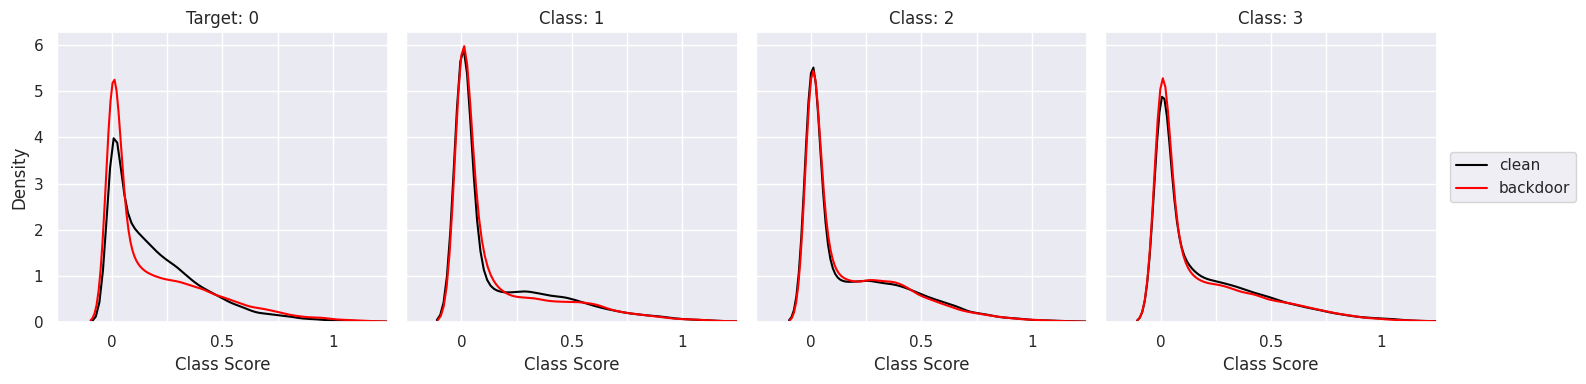
\includegraphics[width=\textwidth]{make_article/make_visuals/visuals/ext_motivation.png}
        \vspace{-10pt}
    \caption{\footnotesize Final hidden layer output distributions (kernel density estimation based) for a {\color{red}\bf backdoor} model (red) and a {\bf clean} model (black). There is an obvious difference between the distributions of the backdoor and clean models for the target label class.}
    \label{fig: motivation}
    \vspace{-5pt}
\end{figure}

\textbf{Detection Framework.} We assume that there exists a small clean validation data set that can be used for gatekeeping the global model for updates. Note that this data set can either belong to a trustworthy existing user or be collected by the centralized server and treated as a new user. Hence, we will refer to this trusted validation data as the trusted user. The detection method leverages the trusted user to evaluate incoming model weights and determine whether each contribution is allowed to participate in the global model update procedure. The main idea is to detect user models with an unusually distributed output layer using information from the trusted user. Our method can be easily extended when several trustworthy data sets or users are present.

\begin{figure}[htp]
\vspace{-5pt}
    \centering
    \adjincludegraphics[page=2, width=\textwidth,trim={0 0 {.1\width} 0}, clip, right]{make_article/make_visuals/extra/extra-figures.pdf}
    \vspace{-15pt}
    \caption{Diagram Representation Of Our Trusted Aggregation Detection Framework.}
    \label{fig: diagram}
    %\vspace{-5pt}
\end{figure}


See Figure~\ref{fig: diagram} for an overview of our proposed detection framework. In each communication round, this validated user completes the following steps to generate a threshold for malicious user detection. First, the validation data is used to update a copy of the global model simultaneous to the local training of other users. When models are returned by the subset of users chosen to potentially participate in the update of the global model, all models, including the validation user and the global model, have predicted scores made and stored for the validation data. We denote the stored predicted scores as $\vo_G, \vo_T$, and $\vo_j$ for the global, validation, and jth user models, respectively.

Next, we compute the distance between the trusted and user models from the global model. Specifically, for each class c, we compute the class-conditional distributional distance $\mathcal{D}(v^{(c)}_j, v^{(c)}_T)$ between the global model output ($\vo^{(c)}_G$) and the user output ($\vo^{(c)}_j$ or $\vo^{(c)}_T$) by applying a distributional difference function. In our experiments, we use the Kolmogorov-Smirnov (KS) distance from estimated CDFs based on $\vo^{(c)}_G$, $\vo^{(c)}_j$, and $\vo^{(c)}_T$. However, we believe there may be other applications where other distance functions should be successful as well. Suppose there are $m$ classes in total; the process will result in a distance vector ($\vv_j, \vv_T\in\sR^m$) for each user, including the trusted user. The distance vectors will then be used to determine which users can participate in the update. Further details are given in Algorithm~\ref{alg:t-agg}. 

\begin{algorithm}[H]
\caption{Trusted Aggregation \\ 
Notation: Let ${\bm S}$ represent the random subset of users that will submit locally trained models $U_j$ to update the global model $G$, $U_T$ to denote the model from the trusted user, $\mX$ to denote the local data of the trusted user, $\mathcal{D}$ to represent the distributional difference function, and $\theta \in [1, 2]$ for the method's scaling coefficient.
}
\label{alg:t-agg}
\begin{algorithmic}[1]

    \Procedure{Trusted Aggregation}{$\mX, G, U_T, \{U_j\}_{j \in {\bm S}}, \theta$}
        %\State Get the local data $\mX$ from the trusted user
        \State Generated outputs: $\vo_G = G(\mX)$, $\vo_{T} = U_T(\mX)$, and $\vo_j = U_j(\mX)$, $\forall j \in \mS$
        \For{each class $c\in [1,...,m]$}
            \State Compute the distributional distances between each user and the global model
            \State \quad $v^{(c)}_T = \mathcal{D}(\vo^{(c)}_G, \vo^{(c)}_T)$ and $v^{(c)}_{j} = \mathcal{D}(\vo^{(c)}_G, \vo^{(c)}_{j})$, $\forall j \in \mS$
            \Comment{$\vo^{(c)}$: output for class $c$}
        \EndFor
        \State The above procedure produces: $\vv_T\in\sR^m, \vv_j\in\sR^m$
        \Comment{$m$: total number of classes}
        \State Compute threshold: $\tau_r = \theta \times\max ( \vv_T )$
        \Comment{$\max$: maximum element of the vector}
        \State  $\tilde{\tau} \gets \Call{Global-Min Mean Smoothing}{\tau}$  \Comment{Algorithm \ref{alg: smoothing}}
        \State Select users: $\mS_r = \{j \in \mS | \max(\vv_{j}) < \tilde{\tau} \}$
        \State \Return FedAvg$(\{U_j\}_{j \in {\bm S}_r})$ 
    \EndProcedure
\end{algorithmic}
\end{algorithm}

\vspace{-10pt}
\textbf{Threshold Construction.} In this part, we discuss how to decide the threshold ($\tau$) and how to use it to select users. We define the true threshold as the largest possible change a non-malicious user could contribute. Users with distance values exceeding the threshold should be excluded. Assume that the class-conditional distances ($v^{(c)}$) are Uniform on $[0, b_c]$ for each class $c$, where $b_c$ is the maximum possible change to the output layer of class $c$ through local training by a non-malicious user. Hence, estimating the threshold consists of estimating the maximum of $b_c$ for any class.  Let $m$ represent the total number of classes. Proposition~\ref{prop: simple} gives simple bounds for our quantity of interest under arbitrary dependence. Therefore, we parameterize our method by $\theta \in [0, 1]$, see Algorithm~\ref{alg:t-agg}.

\vspace{-5pt}
\begin{prop}
\label{prop: simple}
    If $v^{(c)} \sim \text{Uniform}(0, b_c), \forall c \in [1, \ldots, m]$ \text{then} $E \left[ V \right] \leq b_j \leq E \left[ 2 V \right]$ where $V = \max_c v^{(c)}$ and $j = \argmax_c(b_c)$. Proof in Appendix~\ref{app: simple}.
\end{prop}
\vspace{-5pt}

We recommend choosing $\theta$ based on the setting's prevalence of backdoor attacks and the cost of a successful attack to interested parties. For example, twice the maximum of the class-conditional distance ($2V$) is the upper bound for the maximum of $b_c, \forall c\in [1,...,m]$. Such scaling would allow more users to update the global model but increase the risk of a successful backdoor attack. Conversely, using $V$ without scaling would help to prevent stronger backdoor attacks, but with the potential loss of denying benign users from updating the global model. The goal is to choose the smallest $\theta$ that allows benign users to sufficiently create a robust shared machine learning model.

If we additionally assume independence between the class conditional distances, we can establish an additional lower bound, Proposition~\ref{prop: indep}, for our largest possible benign change. Note, Proposition~\ref{prop: indep} converges asymptotically to the earlier lower bound as the size of the classification problem ($m \rightarrow \infty$) grows. Hence, this additional bound is provided to assist with choosing an appropriate $\theta$ for smaller-way classification problems. 

\vspace{-5pt}
\begin{prop}
\label{prop: indep}
    If $v^{(c)} \overset{\indep}{\sim} \text{Uniform}(0, b_c), \forall c \in [1, \ldots, m]$ then $E \left[ \left( \dfrac{m + 1}{m} \right) V \right] \leq b_j$ where $V = \max_c v^{(c)}$ and $j = \argmax_c(b_c)$. Proof in Appendix~\ref{app: indep}.
\end{prop}
\vspace{-5pt}

Since the validated user is non-malicious, their distance vector serves as a good representation for other non-malicious users. Therefore, we estimate the threshold $\tau$ with $\theta\times\max(\vv_T)$, where $\vv_T\in\sR^m$ is the distance vector of the validation user and $\max(\cdot)$ means getting the maximum value of the vector $\vv_T$. Then, the maximum distance value ($\max(\vv_j)$) of each selected user will be compared with the threshold ($\tau$) to determine the final list of users who can participate in the update. A user with a maximum distance smaller than the threshold is considered a benign user, while a user with a maximum distance larger than or equal to the threshold will be removed. However, this naive threshold is very unstable as a lucky malicious user can get past it in some rounds due to the instability. Therefore, we make an additional modification, {\bf global-min mean smoothing}, to this basic threshold to address the concern.


\textbf{Global-Min Mean Smoothing.} A naive way to stabilize the threshold value is using a smoothing method, like a moving average. However, in the early communication rounds, the naive threshold value rapidly decreases as the model starts making connections between inputs and output classes. Therefore, applying a traditional smoothing method can result in a relatively high threshold early, which may let attackers bypass it. When the naive threshold ($\tau$) decreases rapidly, we do not wish to use any previous communication rounds for the smoothing. 

% \pagedepth\maxdimen
\begin{wrapfigure}{r}{.4\textwidth}
\vspace{-5pt}
    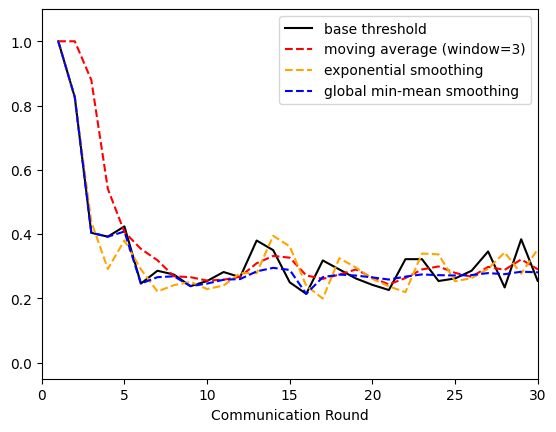
\includegraphics[width=.4\textwidth]{make_article/make_visuals/visuals/smoothing--d_rounds30.png}
    \vspace{-10pt}
    \caption{\footnotesize Comparison of the global min-mean smoothing with the base (naive) threshold and various smoothing methods. 
    %The global min-mean is smooth and captures the early round behavior of the base threshold.
    }
    \label{fig: smoothing}
\end{wrapfigure}

Therefore, we propose to use the lowest observed value (Global Min) of $\tau$ as the starting point of the smoothing window. Let $\tau_t$ represent the naive estimation of the threshold in round $t$. Then the smoothed threshold $\tilde{\tau}$ at round $n$ is given by
\begin{align*}
    \tilde{\tau} = \frac{1}{n-t_s+1}\sum_{t=t_s}^n \tau_t,
\end{align*}
where $t_s$ is the round that when the global min is observed. Details of the global-min mean smoothing are described in Algorithm~\ref{alg: smoothing}. As $\tau_t$ shrinks, we observe new global minimums, and the start of the threshold smoothing is reset.  In addition, when our estimates do not continue to fall, previous values are leveraged to smooth the cutoff, which keeps lucky malicious users from getting past a volatile threshold. Figure~\ref{fig: smoothing} compares our global min-mean smoothing with the naive threshold and various smoothing techniques. The global min-mean smoothing best captures the naive threshold's early behavior while providing remarkable stability improvements. Most importantly, when our threshold encounters a new global minimum, it provides a conservative estimate to prevent malicious users while re-learning cutoff behavior over the next few rounds.

\begin{algorithm}[H]
\caption{Global-Min Mean Smoothing \\ 
Notation: Let $(\tau_1, \cdots, \tau_{n - 1}, \tau_n)$ denote the sequence of values that we wish to smooth.
}
\label{alg: smoothing}
\begin{algorithmic}[1]

    \Procedure{Global-Min Mean Smoothing}{$\tau_1, \cdots, \tau_{n - 1}, \tau_n$}
        \State Record the location of global minimum: $i = \argmin\limits_{t \in [1,...,n] } \tau_t$
        \State Subset to a sequence starting with the global min: $\{\tau_t\}_{t=i}^n = \{\tau_i, \cdots, \tau_n \}$
        \State \Return average of sequence subset, $\overline{\{\tau_t\}_{t=i}^n}$
    \EndProcedure
\end{algorithmic}
\end{algorithm}

\vspace{-5pt}
\section{EXPERIMENTS}

\subsection{Setting}

\textbf{Federated Learning.} We start by giving further specifications regarding the federated learning environment. Our interest is training a global model over $M$ communication rounds with $N$ users. Each iteration randomly selects $K$ users, using a specified proportion of the total users, to participate in the model update. After local training, the next global model is the average returned model weights by the FedAvg procedure. We use ResNet18, a popular classifier proposed in~\cite{resnet}, in all our experiments. We assume that all users, including malicious, have complete control over all aspects of local training, such as learning rate, the number of epochs, and the model weights they return. For simplicity, we select two main sets of training hyper-parameters for benign and malicious users. The malicious users will poison a given proportion of their local data by adding their backdoor trigger to the input and changing the training label to the target class. They intend for the model to associate the trigger with the target class and hence have the future global model identify any input with the trigger as belonging to the target class. 

\textbf{Attack and Baseline.} To show the effectiveness of our method, we choose a setting in which the backdoor attack is strong. We force all malicious users to be included in the subset of selected users to update the global model each round after the start of the backdoor attack. Note that the selection of random users is a defense against malicious users by making it difficult for them to update the global model repeatedly. Additionally, we do not allow the validation user, a guaranteed benign user, to participate in any global model updates. We make these decisions to highlight the ability of our threshold to prevent even unreasonably strong backdoor attacks against the global model. For our experiment, we test the proposed method and two other robust aggregation methods, Median and Trim-mean~\citep{trim-mean}, against two state-of-the-art backdoor attacks in FL: Neurotoxin~\citep{neurotoxin} and Distributed Backdoor Attacks (DBA)~\citep{dba}. To further evaluate the effectiveness of the aggregation methods, we also vary the proportion of malicious attackers to comprise between 10\% and 40\% of the selected users to test the defense methods under different attack strength levels.

\textbf{Data.} The experiments are done on three different data sets: CIFAR10~\citep{krizhevsky2009learning}, STL10~\citep{coates2011analysis} and CIFAR100~\citep{krizhevsky2009learning}. In each experiment, we construct user data sets by random sampling from the training data. For global model evaluation, we split the test set into two parts. We add the backdoor trigger to images in the second half and remove any target class observations. We measure model performance on the first half using {\color{blue}classification accuracy}, and the proportion of the poisoned half predicted as the target class, known as {\color{red}attack success rate}, to measure the extent that the backdoor attack has compromised the model. For a defense method, a good performance consists of a low attack success rate and high classification accuracy. In other words, attacks are unsuccessful when the defense method is used, and the defense does not negatively influence the classification performance. 


\subsection{Main Results}

We begin by considering a setting where 10\% of the selected users are malicious each communication round. Figure~\ref{fig: accuracy--n_malicious1} shows the performance of the three robust aggregation methods against backdoor attacks with and without the Neurotoxin projection on three data sets regarding model classification accuracy and attack success rate. For our main results, we use the TAG scaling coefficients ($\theta$'s) of 2, 2, and 1.1 for the data sets CIFAR10, CIFAR100, and STL10, respectively. Our proposed method nullifies the backdoor attack in each case without decreasing the classification accuracy of the original task in general. We see a slight improvement in classification accuracy for the CIFAR10 data set and a mild decrease in performance on STL10 under the Neurotoxin attack. However, the other two robust aggregation methods, coordinate-wise Median and Trim-mean, fail to prevent backdoor attacks with or without Neurotoxin. We conclude that our method is a clear improvement to the existing robust aggregation methods for federated learning. 

\begin{figure}[htp]
\centering
  \begin{subfigure}{\textwidth}
  \centering
    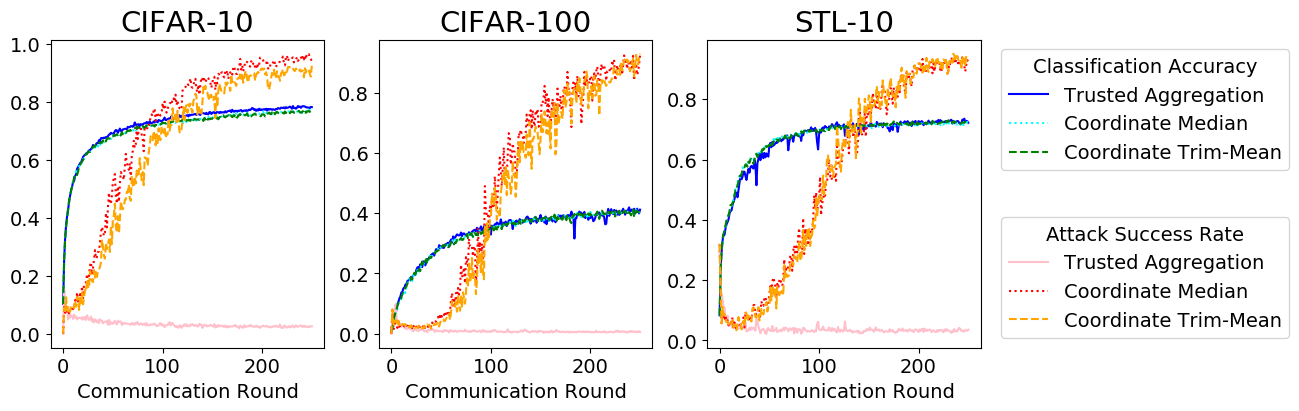
\includegraphics[height=3cm, width=\textwidth]{make_article/make_visuals/visuals/accuracy--n_malicious1--dba0--beta0.2--d_scale.png}
    \caption{\footnotesize Performance Under Backdoor Attack With 10\% Malicious Users.}
  \end{subfigure}%

  \begin{subfigure}{\textwidth}
  \centering
    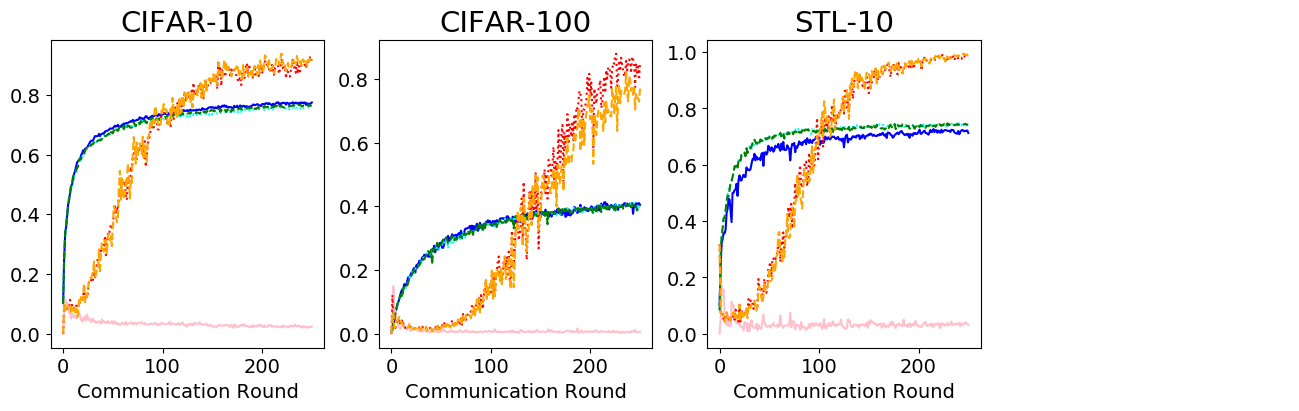
\includegraphics[height=3cm, width=\textwidth]{make_article/make_visuals/visuals/accuracy--n_malicious1--dba0--beta0.2--d_scale--neuro_p0.1_nolegend.png}
    \caption{\footnotesize Performance Under Neurotoxin Backdoor Attack With 10\% Malicious Users.}
  \end{subfigure}%
\caption{\footnotesize Model performance under standard and Neurotoxin backdoor attacks with 10\% malicious users. The proposed method TAG performs well in defending against backdoor attacks as the attack success rates are low. Meanwhile, it does not generally affect the model's classification performance on clean data, except for a slight decrease for the Neurotoxin attack on STL10. However, the other two aggregation methods do not work well against any backdoor attacks.} 
\label{fig: accuracy--n_malicious1}
\end{figure}

We show that TAG can handle even stronger attack settings against state-of-the-art attacks in the following parts. First, we consider testing the robust aggregation methods against DBA and Neurotoxin attacks with 20\% malicious users in the selected set. Unsurprisingly, the robust aggregation methods, which failed against the previous setting, cannot prevent stronger attacks, see Figure~\ref{fig: accuracy--n_malicious2}. On the other hand, our method, TAG, again prevents all backdoor attacks.

\begin{figure}[htp]
\centering
  \begin{subfigure}{\textwidth}
  \centering
    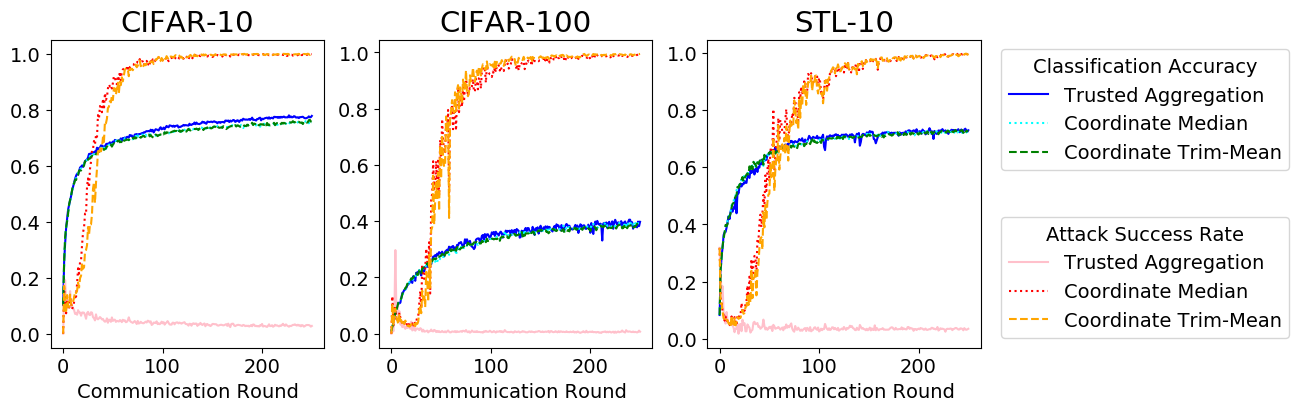
\includegraphics[height=3cm, width=\textwidth]{make_article/make_visuals/visuals/accuracy--n_malicious2--dba1--beta0.2--d_scale.png}
    \caption{\footnotesize Performance Under Backdoor Attack With 20\% Malicious Users.}
  \end{subfigure}%

  \begin{subfigure}{\textwidth}
  \centering
    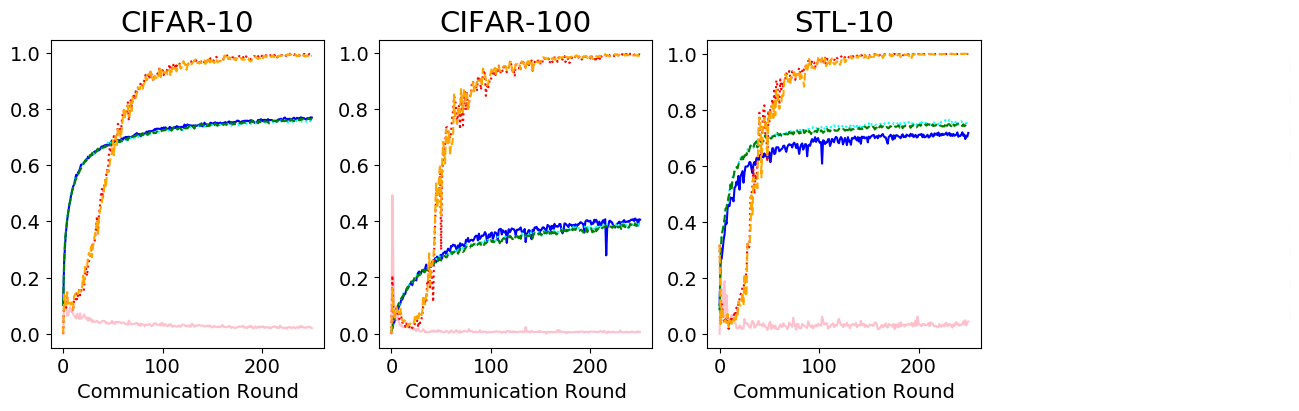
\includegraphics[height=3cm, width=\textwidth]{make_article/make_visuals/visuals/accuracy--n_malicious2--dba1--beta0.2--d_scale--neuro_p0.1_nolegend.png}
    \caption{\footnotesize Performance Under Neurotoxin Backdoor Attack With 20\% Malicious Users.}
  \end{subfigure}%
\caption{\footnotesize Model performance under standard and Neurotoxin backdoor attacks with 20\% malicious users. TAG is the only method that prevents these backdoor attacks.} 
\label{fig: accuracy--n_malicious2}
\end{figure}

Then, we attempt to test our proposed method's limitations by considering DBA and Neurotoxin attacks with 40\% malicious users in the selected set.  These attacks are catastrophically successful against the current robust aggregation methods, see Figure~\ref{fig: accuracy--n_malicious4}, having a nearly perfect attack success rate after round 50 on all our data sets. However, our method, TAG, overcomes the backdoor extent of the initial rounds to prevent the attack against all data sets. Hence, we conclude that even when the federated learning setting updates consist of almost half malicious users, we can use TAG to attempt to eliminate backdoor attacks.

\begin{figure}[htp]
\centering
  \begin{subfigure}{\textwidth}
  \centering
    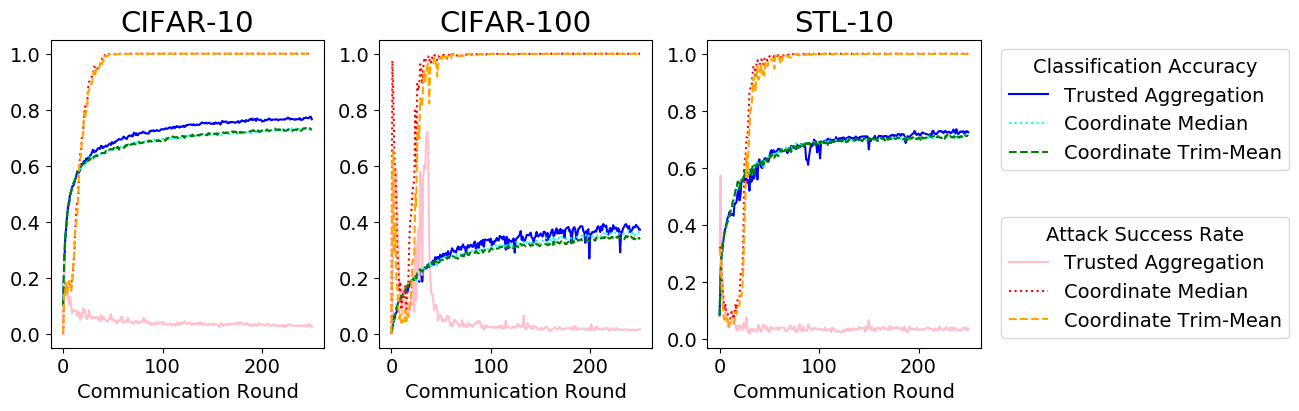
\includegraphics[height=3cm, width=\textwidth]{make_article/make_visuals/visuals/accuracy--n_malicious4--dba1--beta0.2--d_scale.png}
    \caption{\footnotesize Performance Under DBA Backdoor Attack With 40\% Malicious Users.}
  \end{subfigure}%

  \begin{subfigure}{\textwidth}
  \centering
    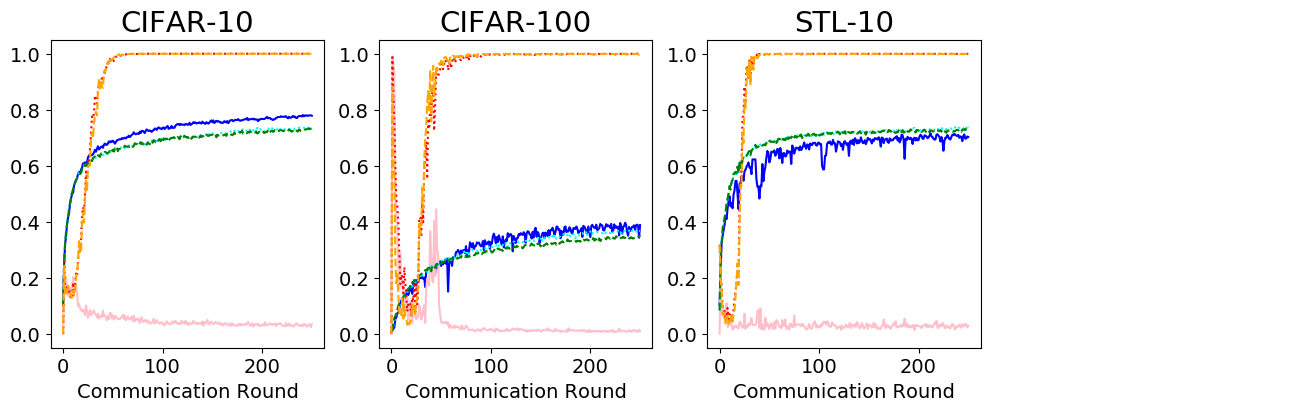
\includegraphics[height=3cm, width=\textwidth]{make_article/make_visuals/visuals/accuracy--n_malicious4--dba1--beta0.2--d_scale--neuro_p0.1_nolegend.png}
    \caption{\footnotesize Performance Under DBA And Neurotoxin Backdoor Attacks With 40\% Malicious Users.}
  \end{subfigure}%
\caption{\footnotesize Model performance under DBA and Neurotoxin backdoor attacks with 40\% malicious users. Again, TAG is the only method that can prevent backdoor attacks.}
\label{fig: accuracy--n_malicious4}
\end{figure}


%
\subsection{Necessity Of Global-Min Mean Smoothing}

We revisit the last attack considered on the STL10 data set to highlight the importance of our proposed technique, global-min mean smoothing. Recall that our smoothing is intended to improve the stability of our estimated threshold while preserving its behavior in the initial rounds, not conserved by other smoothing techniques. If we repeat the backdoor attack where 40\% of the user subset is malicious each round and omit the global-min mean smoothing, our method no longer can prevent these backdoor attacks, see Figure~\ref{fig: accuracy--n_malicious4--no_smooth}. Here our method succumbs to the backdoor attack nearly as quick as the baseline robust aggregation methods. Hence, without global-min mean smoothing, we conclude the malicious users may have a larger opportunity to get past an unstable cutoff.

\begin{figure}[htp]
\centering
  \begin{subfigure}{.35\textwidth}
    \adjincludegraphics[height=4cm,trim={0 0 {.45\width} 0}, clip, right]{make_article/make_visuals/visuals/accuracy--stl_10--n_malicious4--dba1--beta0.2--no_smooth.png}
  \end{subfigure}%
  ~
  \begin{subfigure}{.65\textwidth}
    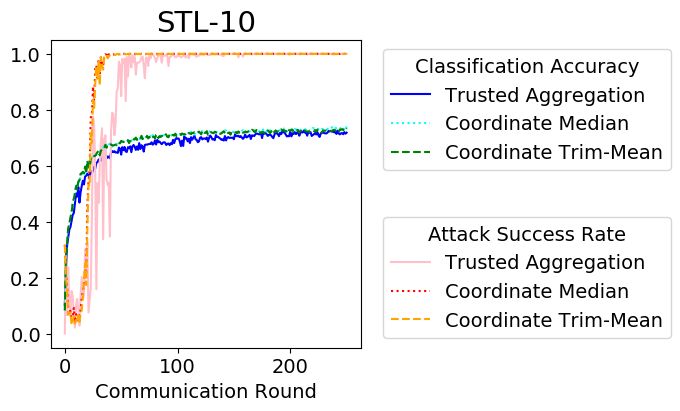
\includegraphics[height=4cm, left]{make_article/make_visuals/visuals/accuracy--stl_10--n_malicious4--dba1--beta0.2--neuro_p0.1--no_smooth.png}
  \end{subfigure}
\caption{\footnotesize Model performance under DBA without (\textit{left}) and with (\textit{right}) Neurotoxin backdoor attacks with 40\% malicious users on STL10 without using global-min mean smoothing. TAG fails to defend against the backdoor attack on STL10 without the improved stability of our estimate from our proposed smoothing technique, global-min mean smoothing.}
\label{fig: accuracy--n_malicious4--no_smooth}
\end{figure}


%
\subsection{Data Distribution Study}

In this section, we show the applicability of our method for imbalanced users focusing on the CIFAR10 data set. Recall that local data sets are not required to be independent and identically distributed for federated learning. For our experiments, the user data sets are obtained by random sampling from the training data. In this experiment, we use the m-dimensional (number of total classes) Dirichlet distribution to determine the proportion for each class to be randomly sampled. We parameterize this distribution by the simplified $\alpha \mathbf{1}_m$ where $\mathbf{1}_m$ is an m-dimensional vector of ones, and $\alpha \in [0, \infty)$ is a scalar such that smaller values lead to imbalanced user data.

\begin{figure}[htp]
\centering
  \begin{subfigure}{.35\textwidth}
  \centering
    \adjincludegraphics[height=4cm,trim={0 0 {.45\width} 0}, clip, right]{make_article/make_visuals/visuals/accuracy--cifar_10--n_malicious4--dba1--beta0.2--d_scale1.25--alpha1.png}
  \end{subfigure}%
  ~
  \begin{subfigure}{.65\textwidth}
  \centering
    \adjincludegraphics[height=4cm, trim={0 0 0 0}, clip, left]{make_article/make_visuals/visuals/accuracy--cifar_10--n_malicious4--dba1--beta0.2--d_scale1.5--neuro_p0.1--alpha1.png}
  \end{subfigure}%

\caption{\footnotesize Model performance under DBA without (\textit{left}) and with (\textit{right}) Neurotoxin backdoor attacks with 40\% malicious users on imbalanced local user data sets. The proposed method, TAG, performs well in defending against backdoor attacks for all data sets, even when the user data is randomly sampled using the Dirichlet distribution with $\alpha = 1$. However, for the extreme case with 40\% malicious, the scaling parameter for TAG, $\theta$, needed to be reduced to prevent stronger attacks. Again, the other two aggregation methods do not work well in preventing any backdoor attack under imbalanced data.}
\label{fig: accuracy--n_malicious4--alpha1}

\end{figure}


\yli{Regarding attacks with 10\% and 20\% malicious users, we did not have to modify the scaling parameter $\theta$ from previously balanced data experiments to have a successful defense when data is highly imbalanced ($\alpha = 1$), see results in Figure~\ref{fig: accuracy--n_malicious2--alpha1} and Figure~\ref{} (10\% Figure?) in Appendix.}
Our method prevents such backdoor attacks while achieving great classification accuracy for the original task. This setting alone is more than sufficient to show the usefulness of our proposed method TAG in the majority of federated learning settings.

Furthermore, TAG is successful against the unreasonably strong 40\% malicious setting if we reduce the scaling coefficient $\theta$. Recall the trade-off between robustness against backdoor attacks and performance for the original classification task. In Figure~\ref{fig: accuracy--n_malicious4--alpha1}, with $\theta=1.25$ and $\theta=1.5$ respectively, TAG is able to eliminate the backdoor attacks. With smaller scaling, the original classification accuracy suffers in early communication rounds. However, as the global model nears convergence, the round-to-round accuracy stabilizes and becomes equal to or better than the baseline robust aggregation methods. Hence, we conclude that our proposed method, TAG, can handle backdoor attacks on reasonably imbalanced data without losing accuracy for the original task. These experiments support our recommendation to choose the smallest scaling possible that achieves desired performance on the original task to prevent backdoor attacks.


\begin{figure}[htp]
\centering
\end{figure}




%
\subsection{Validation User Data Proportion Study}

For previous experiments, we have assumed that the validation user has a data set of the same size as the other users. In most cases, data can be acquired. However, we want to determine whether our method depends on such size requirements. Hence we revisit the strongest attack setting for the CIFAR10 data set but only allow the validation user to have a data set that is 20\% of the size of the other local users. Here the validation set is now only allowed 100 images, yet TAG prevents the backdoor attack and can achieve improved accuracy compared to the baseline robust aggregation methods. Hence, we conclude we do not need validation data of the same quantity as other local users to discriminate between benign and malicious returning models.

\begin{figure}[htp]
\centering
  \begin{subfigure}{.35\textwidth}
  \centering
    \adjincludegraphics[height=4cm,trim={0 0 {.45\width} 0}, clip, right]{make_article/make_visuals/visuals/accuracy--cifar_10--n_malicious4--dba1--beta0.2--n_val_data100.png}
  \end{subfigure}%
  ~
  \begin{subfigure}{.65\textwidth}
  \centering
    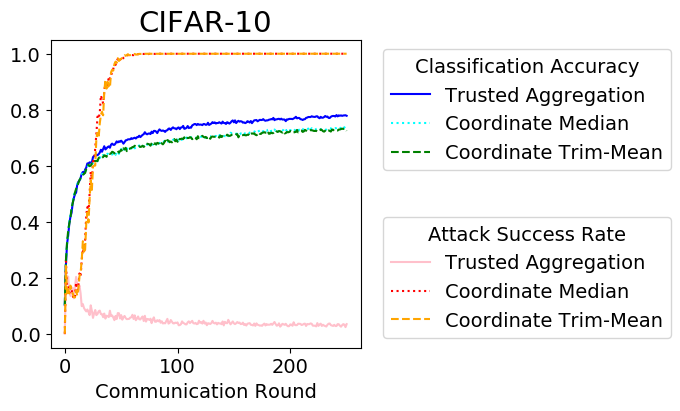
\includegraphics[height=4cm, left]{make_article/make_visuals/visuals/accuracy--cifar_10--n_malicious4--dba1--beta0.2--neuro_p0.1--n_val_data100.png}
  \end{subfigure}%
\caption{\footnotesize Model performance under DBA and Neurotoxin backdoor attacks with 40\% malicious users on CIFAR10 where the validation data set is 20\% the size of the local users. Still, the proposed method TAG performs well, and the other two aggregation methods do not work well in preventing any backdoor attack.}
\label{fig: accuracy--n_malicious4--n_val_data100}
\end{figure}


% 
\section{Conclusion}

While current robust aggregation methods fail to prevent mild backdoor attacks, TAG holds up against state-of-the-art attacks in unreasonably strong settings. Furthermore, TAG works when users have heterogeneous and imbalanced data, does not decrease the classification accuracy for the original task, and only a minimal validation set is required. Finally, TAG is compatible with other filtering methods or modifications to the choice of aggregation step. We believe our proposed method, Trusted Aggregation (TAG), is an essential advancement toward model security for the federated learning framework.

\newpage
{  \small 
\bibliographystyle{iclr2023_conference}
\bibliography{iclr2023_conference}
}


%
\pagebreak\appendix

\section{Supplementary Results}

%
\subsection{Model Performance When No Backdoor Attack}

%
\subsection{Additional Figures For Data Distribution Study}

\begin{figure}[htp]
  \begin{subfigure}{.35\textwidth}
  \centering
    \adjincludegraphics[height=4cm,trim={0 0 {.45\width} 0}, clip, right]{make_article/make_visuals/visuals/accuracy--cifar_10--n_malicious2--dba1--beta0.2--alpha1.png}
  \end{subfigure}%
  \begin{subfigure}{.65\textwidth}
  \centering
    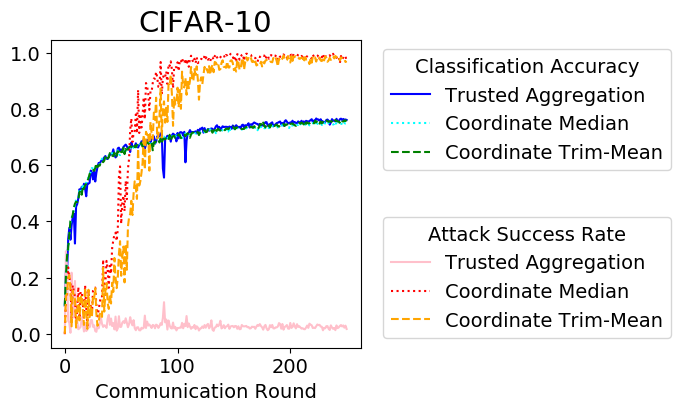
\includegraphics[height=4cm, left]{make_article/make_visuals/visuals/accuracy--cifar_10--n_malicious2--dba1--beta0.2--neuro_p0.1--alpha1.png}
  \end{subfigure}%
\caption{\footnotesize Model performance under DBA without (\textit{left}) and with (\textit{right}) Neurotoxin backdoor attacks with 20\% malicious users on imbalanced local user data sets. The proposed method, TAG, performs well in defending against backdoor attacks for all data sets, even when the user data is randomly sampled using the Dirichlet distribution with $\alpha = 1$ without changing the scaling parameter ($\theta$). Again, the other two aggregation methods do not work well in preventing any backdoor attack under imbalanced data.}
\label{fig: accuracy--n_malicious2--alpha1}

\end{figure}


\section{Supplementary Proofs}
\subsection{Proof of Proposition \ref{prop: simple}}
\label{app: simple}
\begin{align*}
    & \textrm{Assume } \forall c \in [1,...,m], v^{(c)} \sim \textrm{ Unif}(0, b_c) \\
    & \textrm{Define } V = \max_c \left( v^{(c)} \right) \textrm{ and } j = \argmax_c (b_c) \\
    & \quad v^{(j)} \leq V \leq b_j \Longrightarrow E \left[ v^{(j)} \right] = \dfrac{b_j}{2} \leq E \left[ V \right] \leq b_j  \Longrightarrow E \left[ V \right] \leq b_j \leq E \left[ 2 V \right]
\end{align*}

\subsection{Proof of Proposition \ref{prop: indep}}
\label{app: indep}
\begin{align*}
    & \textrm{Assume } \forall c \in [1,...,m], v^{(c)} \overset{\textrm{ind}}{\sim} \textrm{ Unif}(0, b_j) \\
    & \quad \textrm{Let } W = \max_c \left( w^{(c)} \right) \textrm{ where } w^{(c)} \overset{\textrm{iid}}{\sim} \textrm{ Unif}(0, b_j) \Longrightarrow \dfrac{W}{b_j} \sim \textrm{Beta}(m, 1) \Longrightarrow E(W) = \dfrac{m}{m + 1} \\
    & \quad F_V(t) = P(V \leq t) = \prod_{i = 1}^m P_{v^{(c)}}(t) \geq \prod_{i = 1}^m P_{w^{(c)}}(t) = P(W \leq t) = F_W(t) \\
    & \quad \Longrightarrow E(V) = \int_0^\infty (1 - F_V(t)) \,dt \leq \int_0^\infty (1 - F_W(t)) \,dt = E(W) \\
    & \quad \Longrightarrow E \left[ \dfrac{V}{b_j} \right] \leq E \left[ \dfrac{W}{b_j} \right] = \dfrac{m}{m + 1} \Longrightarrow E \left[ \left( \dfrac{m + 1}{m} \right) V \right] \leq b_j \\
    \nonumber 
\end{align*} 



\end{document}
